\documentclass[a4paper,12pt,frenchb]{article}

\input{../../commons.tex.inc}

\title{Évaluation : géométrie dans l'espace}
\author{semaine \no{47} -- 10\up{ième} semaine de cours}
\date{20 novembre 2017}

\SetWatermarkText{}
\parindent0pt

\begin{document}


\maketitle

\thispagestyle{fancy}

\begin{question}[subtitle={septembre 2016, antilles-guyanne, 2 points}]

  On considère un cube $ABCDEFGH$ de côté 1.

  \begin{center}
    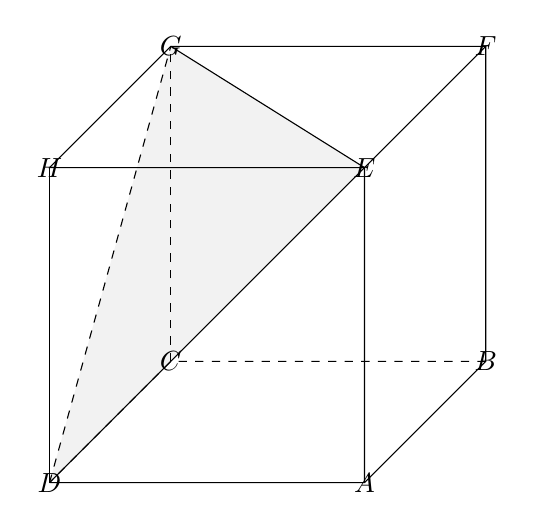
\begin{tikzpicture}[scale=4]
      \fill[gray!10!white] (0,0,1) -- (1,1,1) -- (0,1,0) ;
      \draw [dashed] (0,0,1) -- (0,1,0) ;
      \draw (0,1,0) -- (1,1,1) -- (0,0,1) ;
      \draw (0,0,1) node {$D$} -- (1,0,1) node {$A$} -- (1,1,1) node {$E$}
        -- (1,1,0) node {$F$} -- (0,1,0) node {$G$} -- (0,1,1) node {$H$} --
        (1,1,1);
      \draw (0,1,1) -- (0,0,1) ;
      \draw (1,0,1) -- (1,0,0) node {$B$}-- (1,1,0) ;
      \draw [dashed] (1,0,0) -- (0,0,0) node {$C$} -- (0,0,1) ;
      \draw [dashed] (0,0,0) -- (0,1,0) ;
    \end{tikzpicture}
  \end{center}

  On se place dans le repère $\brk*{B,\vv{BA}, \vv{BC}, \vv{BF}}$.
  \begin{enumerate}
    \item Déterminer une équation de la droite $(BH)$.

      On admet que \[ (DF) : \left\{ \begin{matrix} x= 1 - s & \\ y = -s ,&
      s \in \R \\ z = s & \\ \end{matrix} \right. . \]
    \item Donner les coordonnées du point $P$, point d'intersection des
      droites $(BH)$ et $(DF)$.
    \item Que représente le point $P$ pour le triangle $DEG$ ? Justifier la
      réponse.
  \end{enumerate}
\end{question}

\begin{question}
  Dériver les fonctions suivantes.

  \begin{enumerate}
    \item $f \colon x \mapsto \frac1{(x+2)^2}$.
    \item $g \colon x \mapsto \frac{x^3}4 -x + \frac38$.
    \item $h \colon x \mapsto x + \frac{765}x$.
  \end{enumerate}
\end{question}

\end{document}
